\documentclass[letterpaper, 12pt]{article}

%%%%%%%%%%%%%%%%%%%%%%%%%%%%%
% DEFINITIONS
% Change those informations
% If you need umlauts you have to escape them, e.g. for an ü you have to write \"u
\gdef\mytitle{Übungsprotokoll A04}
\gdef\mythema{Continuous Integration mit Jenkins}

\gdef\mysubject{Softwareentwicklung}
\gdef\mycourse{5BHIT 2017/18}
\gdef\myauthor{Martin W\"olfer}

\gdef\myversion{0.1}
\gdef\mybegin{Begonnen am 5. Oktober 2017}
\gdef\myfinish{Beendet am \today}

\gdef\mygrade{Note:}
\gdef\myteacher{Betreuer: DOLD \& RAFW}
%
%%%%%%%%%%%%%%%%%%%%%%%%%%%%%

%!TEX root=../document.tex

\usepackage[in]{fullpage}
% Fontencoding for possible copy&paste out of PDF
\usepackage[T1]{fontenc}
\usepackage[utf8]{inputenc}
\usepackage[ngerman]{babel}
\usepackage{graphicx} 
\usepackage{wasysym}
\usepackage{textcomp}
\usepackage{sectsty}
\usepackage{caption}
\usepackage{listings}
\usepackage{array}
\usepackage{nonfloat}
\usepackage{colortbl}
\usepackage{footmisc}
\usepackage{fancyhdr}
\usepackage{ccicons}
\usepackage{suffix}
\usepackage{multirow}
\usepackage{tabularx}
\usepackage{listings}
\usepackage{accsupp}
\usepackage{color}
\usepackage{url}
\usepackage[dvipsnames]{xcolor}
\usepackage[longnamesfirst,nonamebreak]{natbib}
\usepackage[headsep=1cm,headheight=3cm,hmargin=2cm,vmargin=2.5cm]{geometry}
\usepackage[nolist]{acronym}

% Definitions for Textcolor
\usepackage{color}
\definecolor{listings}{rgb}{0.96, 0.96, 0.96}
\definecolor{update}{rgb}{1, 0.8, 0.8}
\definecolor{config}{rgb}{0.8, 1, 0.8}
\definecolor{gray}{rgb}{0.4,0.4,0.4}
\definecolor{darkblue}{rgb}{0.0,0.0,0.6}
\definecolor{cyan}{rgb}{0.0,0.6,0.6}

% Java Syntaxhighligthning
% strings
\definecolor{javared}{rgb}{0.6,0,0}
% comments
\definecolor{javagreen}{rgb}{0.25,0.5,0.35}
% keywords
\definecolor{javapurple}{rgb}{0.5,0,0.35}
% javadoc
\definecolor{javadocblue}{rgb}{0.25,0.35,0.75}

\lstset{
	basicstyle=\ttfamily\small,
	keywordstyle=\bfseries\color[rgb]{0.496,0.000,0.332},
	commentstyle=\color[rgb]{0.246,0.496,0.371},
	stringstyle=\color[rgb]{0.164,0.000,0.996},
	tabsize=4,
	breaklines=true,
	numbers=left,
	numberstyle=\tiny\color{black},
	stepnumber=2,
	numbersep=8pt,
	numberstyle=\tiny,
	captionpos=b,
	xleftmargin=1cm,
	showspaces=false,
	showstringspaces=false,
	basewidth={0.53em,0.45em},
	frame=single,
	xleftmargin=1cm,
	basicstyle=\scriptsize,
}


\lstdefinestyle{Java}{
	language=Java,
	keywordstyle=\color{javapurple}\bfseries,
	stringstyle=\color{javared},
	commentstyle=\color{javagreen},
	morecomment=[s][\color{javadocblue}]{/**}{*/},
}

\lstdefinelanguage{XML}
{
	morestring=[b]",
	morestring=[s]{>}{<},
	morecomment=[s]{<?}{?>},
	stringstyle=\color{black},
	identifierstyle=\color{darkblue},
	keywordstyle=\color{cyan},
	% list your attributes here
	morekeywords={xmlns,version,type}
}

\lstdefinestyle{XML}{
	language=XML,
	basicstyle=\ttfamily\small,
	columns=fullflexible,
	commentstyle=\color{gray}\upshape
}

\newcommand{\noncopynumber}[1]{
	\BeginAccSupp{method=escape,ActualText={}}
	#1
	\EndAccSupp{}
}
\lstdefinestyle{bash}{
	language=bash,
	basicstyle=\ttfamily\small,
	literate={-}{{-}}{1},
	% http://tex.stackexchange.com/questions/145416/how-to-have-straight-single-quotes-in-lstlistings
	upquote=true;
	showstringspaces=false,
	%numbers=none,
	% http://tex.stackexchange.com/questions/122256/only-select-code-without-line-numbers
	numberstyle=\tiny\noncopynumber,
	breaklines=false,
	columns=fullflexible,
	basicstyle=\scriptsize
}

% http://tex.stackexchange.com/questions/83085/how-to-improve-listings-display-of-json-files
\colorlet{punct}{red!60!black}
\definecolor{background}{HTML}{EEEEEE}
\definecolor{delim}{RGB}{20,105,176}
\colorlet{numb}{magenta!60!black}
\lstdefinelanguage{json}{
	basicstyle=\ttfamily\small,
	numbers=left,
	numberstyle=\scriptsize,
	stepnumber=2,
	numbersep=8pt,
	showstringspaces=false,
	breaklines=true,
	literate=
	*{0}{{{\color{numb}0}}}{1}
	{1}{{{\color{numb}1}}}{1}
	{2}{{{\color{numb}2}}}{1}
	{3}{{{\color{numb}3}}}{1}
	{4}{{{\color{numb}4}}}{1}
	{5}{{{\color{numb}5}}}{1}
	{6}{{{\color{numb}6}}}{1}
	{7}{{{\color{numb}7}}}{1}
	{8}{{{\color{numb}8}}}{1}
	{9}{{{\color{numb}9}}}{1}
	{:}{{{\color{punct}{:}}}}{1}
	{,}{{{\color{punct}{,}}}}{1}
	{\{}{{{\color{delim}{\{}}}}{1}
	{\}}{{{\color{delim}{\}}}}}{1}
	{[}{{{\color{delim}{[}}}}{1}
	{]}{{{\color{delim}{]}}}}{1},
	basicstyle=\scriptsize
}

\usepackage[
	colorlinks,
	citecolor=black,
	filecolor=black,
	linkcolor=black,
	urlcolor=black,
	linktoc=all
]{hyperref}


\let\tempsection\section
\renewcommand\section[1]{\vspace{-0.3cm}\tempsection{#1}\vspace{-0.3cm}}
\WithSuffix\newcommand\section*[1]{\tempsection*{#1}}

\let\tempsubsection\subsection
\renewcommand\subsection[1]{\vspace{0cm}\tempsubsection{#1}\vspace{0cm}}

\let\tempsubsubsection\subsubsection
\renewcommand\subsubsection[1]{\vspace{0cm}\tempsubsubsection{#1}\vspace{0cm}}

\linespread{0.94}

\lhead{\mysubject}
\chead{}
\rhead{\bfseries\mythema}
\lfoot{\mycourse}
\cfoot{\thepage}
% Creative Commons license BY
% http://creativecommons.org/licenses/?lang=de
\rfoot{\ccby\hspace{2mm}\myauthor}
\renewcommand{\headrulewidth}{0.4pt}
\renewcommand{\footrulewidth}{0.4pt}

\begin{document}
	\parindent 0pt
	\parskip 6pt
	
	\pagenumbering{Roman} 
	%!TEX root=../laborprotokoll.tex

\begin{titlepage}

	\begin{figure}[!h]
		\begin{flushright}
			
\includegraphics[width=0.3\linewidth]{images/jdIT_tgm.png}
		\end{flushright}
	\end{figure}

	\vspace{2.5cm} 

	{\begin{center} \bfseries\huge
			\rule{17.5cm}{0.1mm}  
			\\[5mm]
			\mytitle\\[5mm]
			\mythema\\
			\rule{17.5cm}{0.1mm}  
	\end{center}}

	{\begin{flushright} \bfseries\Large
			\vspace{2cm}
			\mysubject\\
			\mycourse\\[10mm]
			\myauthor\\[10mm]
	\end{flushright}}

	{\begin{table}[!h] \bfseries\normalsize
		\begin{tabularx}{\textwidth}{lXr @{\hspace{0mm}}}
			&& Version \myversion\\
			\mygrade && \mybegin\\
			\myteacher && \myfinish\\
		\end{tabularx}
	\end{table}}

\end{titlepage}

	
	\clearpage
	\thispagestyle{empty}
	\tableofcontents
	
	\newpage
	\pagenumbering{arabic}
	\pagestyle{fancy}
	
	%\vspace{-0.5cm}
	
	%!TEX root=../document.tex
\section{Aufgabenstellung}
\subsection{UML-Klassendiagramm der verwendeten Architektur inkl. Beschreibung}
\subsection{Kurze allgemeine Ausarbeitung zu Design Patterns}
\begin{itemize}
	\item Wie können Design Patterns unterteilt werden
	\item Wozu Design Patterns
	\item Übersicht existierender Design Patterns
\end{itemize}
\subsection{Ausarbeitung zum Decorator Pattern}
\begin{itemize}
	\item Allgemeines Klassendiagramm
	\item Grundzüge des Design Patterns (wichtige Operationen etc.) am Beispiel des implementierten Programms inkl. spezielles Klassendiagramm
	\item Vor- und Nachteile
	\item (Weitere) Anwendungsfälle
\end{itemize}
\subsection{Ausarbeitung zu \textbf{einem} der folgenden Design Patterns: Observer, Abstract Factory, Strategy}
\begin{itemize}
	\item Allgemeines Klassendiagramm
	\item Grundzüge des Design Patterns (wichtige Operationen etc.) mit einem kurzen eigenen Beispiel inkl. spezielles Klassendiagramm
	\item Vor- und Nachteile
	\item (Weitere) Anwendungsfälle
\end{itemize}




\clearpage

	%!TEX root=../document.tex

\section{Installation}
Die Installation von web2py kann in 10 Sekunden erfolgen. Es wird lediglich ein \verb|.zip| heruntergeladen von der
\underline{\href{http://www.web2py.com/init/default/download}{offiziellen Seite}} ($\rightarrow$ \textbf{Source Code}).

Der Source Code wird anschließend, und in diesem Ordner wird mit \textbf{python2} das File \verb|web2py.py| ausgeführt:

\begin{lstlisting}[language=bash]
cd web2py
python2 web2py.py
\end{lstlisting}

Anschließend öffnet sich ein Fenster, bei welchem man angeben kann unter welcher Adresse man die Website und die Datenbank laufen haben will, in dem Anwendungsbeispiel \textbf{localhost}. Weiter kann ein Port ausgewählt werden, über welchem man web2py aufruft, standardmäßig wird der Port \textbf{8000} gewählt. 

Zum Schluss muss noch ein Administrator Passwort gewählt, mit diesem verwaltet man jene Seite, welche momentan mit diesem Server aufgesetzt wird. Wichtig ist, jedes mal wenn der Server neu gestartet wird (d.h. \verb|web2py.py| ausgeführt wird) wird nach einem neuen Passwort gefragt.

\begin{minipage}{\linewidth}
	\centering
	
\includegraphics[width=0.5\linewidth]{images/start}
	\figcaption{web2py grafisches interface}
\end{minipage}

Nun kann \textbf{localhost:8000} aufgerufen werden, und man wird von der Standardseite empfangen.

\section{Generell web2py}
web2py ist ein sehr umfangreiches framework, und das merkt man sofort sobald man die default-seite aufruft. Es gibt sehr viele Optionen und man ist anfänglicher weise leicht überwältigt. Bevor überhaupt daran gedacht werden kann, eine app zu schreiben, muss sich web2py in der Theorie angeschaut werden.

\subsection{Aufbau}
Alle Applikationen in web2py sind mit dem \textbf{MVC-Modell}aufgebaut. Weiters ist wichtig, dass web2py einen Programmierstil voraussetzt, welcher \textbf{''coding-by-convention''} genannt wird. Dies bedeutet, dass der Programmierer sich immer an die Konventionen halten sollte, aber wenn nicht muss er dies explizit angeben. Durch diesen Stil wird dem Softwareentwickler sehr viel arbeit abgenommen weil sehr viele Beziehungen oder sogar Daten automatisch erzeugt werden.

\begin{minipage}{\linewidth}
	\centering
	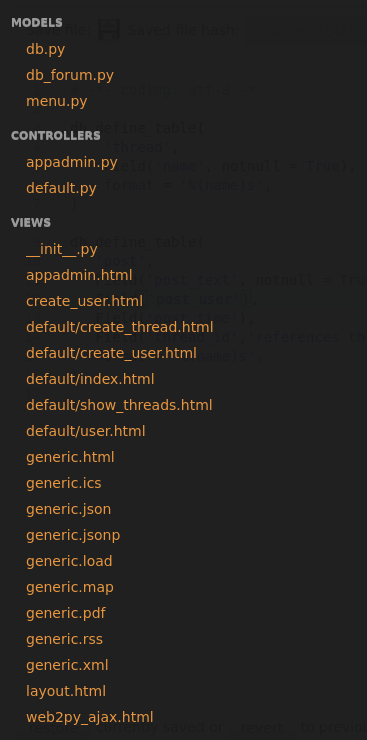
\includegraphics[width=0.45\linewidth]{images/aufbau}
	\figcaption{Grundsätzlicher Aufbau von web2py}
\end{minipage}

\subsection{Model}
In web2py stellt das Model die Datenbank dar. Unter dem Bereich \textbf{Model} können \verb|.py| Files erzeugt werden, in welchem die einzelnen Tabellen definiert werden können. Hierbei wird nicht normales \verb|SQL| geschrieben, sondern es wird die Datenbank Abstraktionsschicht von web2py verwendet, auch \textbf{DAL} (\textbf{D}atabase \textbf{A}bstraction \textbf{Layer}) genannt. Dadurch können \textbf{CRUD} Anweisungen leichter ausgeführt werden.

Natürlich können auch hier, wie in SQL, constraints definiert werden um die Tabellen konsistent zu halten. Wichtig ist nur, dass wie in Django keine \textbf{Primary Keys} definiert werden müssen, da jede Tabelle automatisch ein Feld \textbf{Id} hat, welches automatisch inkrementiert wird mit jeder neuen Reihe. 

Eine Tabelle besitzt folgende Optionen definiert zu werden: 

\begin{lstlisting}[language=python]
db.define_table('person',
	Field('name'),
	id=id,
	rname=None,
	redefine=True
	common_filter,
	fake_migrate,
	fields,
	format,
	migrate,
	on_define,
	plural,
	polymodel,
	primarykey,
	redefine,
	sequence_name,
	singular,
	table_class,
	trigger_name)

\end{lstlisting}

Ein Feld, hat folgende Signatur
\begin{lstlisting}[language=python]
Field(fieldname, type='string', length=None, default=None,
	required=False, requires='<default>',
	ondelete='CASCADE', notnull=False, unique=False,
	uploadfield=True, widget=None, label=None, comment=None,
	writable=True, readable=True, update=None, authorize=None,
	autodelete=False, represent=None, compute=None,
	uploadfolder=None, uploadseparate=None, uploadfs=None, rname=None)
\end{lstlisting}

\clearpage
\subsection{Controller}
In web2py werden vom Controller die User-eingaben verwaltet und weitergeleitet - meistens an die View. Wichtig ist, jede Funktion welche im Controller definiert wird, kann im Browser aufgerufen werden, wahrscheinlich über eine REST-Schnittstelle.

Bsp:

Folgende Funktion wird in \verb|default.py| definiert:

\begin{lstlisting}[language=python]
	def hello_world():
		return "Hello World"
\end{lstlisting}

Liefert folgendes Ergebnis:

\begin{minipage}{\linewidth}
	\centering
	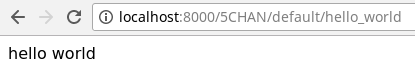
\includegraphics[width=0.45\linewidth]{images/hello_world}
	\figcaption{localhost:8000/app\_name/default/hello\_world}
\end{minipage}

\subsection{View}
Als Model wird in web2py die Darstellung verstanden. Hierbei werden \verb|.html| Dateien erstellt, welche aber durchaus Logik enthalten können, vor allem in Kommunikation mit dem Controller. Die Verwendung von HTML-Dateien in web2py erinnert stark an die Verwendung von \verb|.xhtml| in Java. 

Mit doppelt geschwungenen Klammern können Variablen aufgerufen werden, welche vom Controller in einem \verb|dict| zurückgegeben wurden. Wie in Java, ist es auch hier möglich mit \verb|extends| von einem HTML-File zu erben, um ein bestimmtes Layout über alle Seiten zu besitzen.

Bsp:

Folgende Funktion wird in \verb|default.py| definiert:

\begin{lstlisting}[language=python]
def hello_world():
	return dict(msg="hello_world")	
\end{lstlisting}

Und in \verb|default/hello_world.html| wird folgendes definiert:

\begin{lstlisting}[language=python]
<h1>Vom Controller wurde folgendene Nachricht uebergeben: </h1>
{{=msg}}
\end{lstlisting}

Und dies liefert folgendes Ergebnis:

\begin{minipage}{\linewidth}
	\centering
	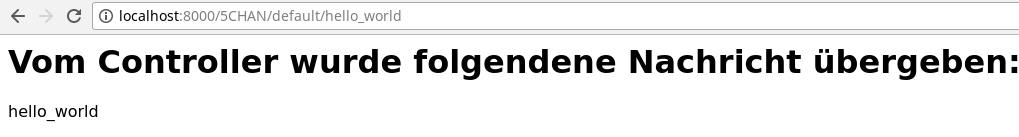
\includegraphics[width=1\linewidth]{images/hello_world2}
\end{minipage}

\section{Anwendungsfall}
Idee ist es, eine sehr vereinfachte Form eines Forums zu programmieren. 

\subsection{Datenbank(Model)}
Zuerst wurde sich ein einfaches Datenbankmodell überlegt, um die Daten abzuspeichern.
\subsubsection{Modellierung}
\begin{minipage}{\linewidth}
	\centering
	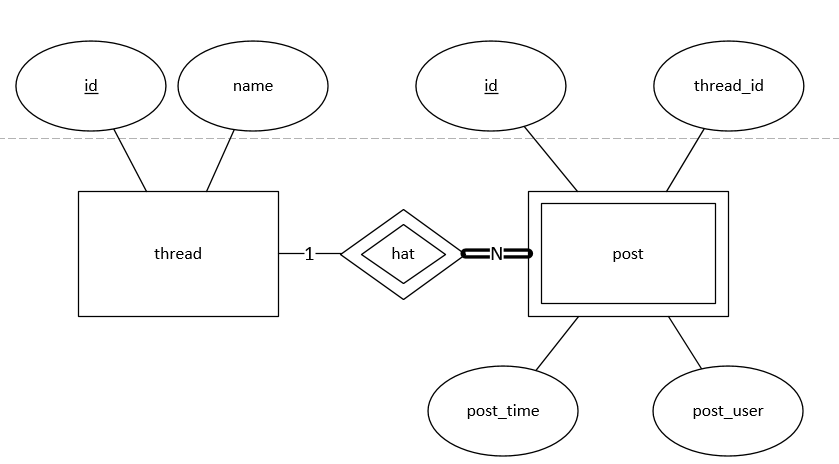
\includegraphics[width=0.8\linewidth]{images/diagram}
	\figcaption{ERD-Diagramm der Datenbank}
\end{minipage}

\subsubsection{Umsetzung}
\begin{lstlisting}[language=python]
db.define_table(
	'thread',
	Field('name', notnull = True),
	format = '%(name)s',
)
	
db.define_table(
	'post',
	Field('post_text', notnull = True),
	Field('post_user'),
	Field('post_time'),
	Field('thread_id','references thread'),
	format = '%(name)s',
)
\end{lstlisting}

\subsection{Controller}
Der Controller nimmt Daten aus der Datenbank und übergibt diese dem View.

In index() wird die Liste der Threads, deren Posts und ein Button zum erstellen eines neuen Threads übergeben.
\begin{lstlisting}[language=python]
def index():
    threads = db(db.thread).select()
    records = SQLFORM.grid(db.thread, db.thread(), deletable=True)
    form = SQLFORM(db.thread).process()
    form.element(_type='submit')['_value'] = T("Thread erstellen")
    posts = db().select(db.post.ALL)
    if form.accepted:
        redirect(URL("index.html"), client_side=True)
        response.flash = T("Neuer Thread wurde erstellt")
    return dict(threads=threads, records=records,form=form, posts=posts)
\end{lstlisting}

Wenn create\_post() aufgerufen wird, fügt es der Datenbank zum jeweiligen Thread den neuen Post hinzu.
\begin{lstlisting}[language=python]
def create_post():
    thread = request.args[0]
    back_button = A(T('Back'), _href=URL('default', 'index', user_signature=True), _class='btn')
    form=SQLFORM(db.post, fields=['post_text','post_user'])
    form.vars.thread_id = thread
    form.process()
    return dict(form=form,thread=thread,back_button=back_button)
\end{lstlisting}

delete\_post() löscht einen bestimmten Post aus einem Thread.
\begin{lstlisting}[language=python]
def delete_post():
    post = request.args[0]
    db(db.post.id==post).delete()
    redirect(URL("index.html"), client_side=True)
\end{lstlisting}

update\_post() lässt einen einen Post bearbeiten.
\begin{lstlisting}[language=python]
def update_post():
    post = request.args[0]
    record = db.post(post)
    form=SQLFORM(db.post, record, fields=['post_text'])
    form.vars.thread_id = request.args[2]
    form.vars.post_user = request.args[1]
    form.process()
    db(db.post.id==request.args[3]).delete()
    back_button = A(T('Back'), _href=URL('default', 'index', user_signature=True), _class='btn')
    return dict(form=form, back_button=back_button)
\end{lstlisting}

delete\_thread() löscht den spezifizierten Thread.
\begin{lstlisting}[language=python]
def delete_thread():
    thread = request.args[0]
    db(db.thread.id==thread).delete()
    redirect(URL("index.html"), client_side=True)
\end{lstlisting}

\subsection{View}
update\_post.html stellt die Daten dar, die es von update\_post() bekommt (Formular und button).
\begin{lstlisting}[language=html]
{{extend 'layout.html'}}
<h1>Einen Post updaten</h1>
{{=form}}
{{=back_button}}
\end{lstlisting}

index.html stellt die Threads und deren Posts Tabelarisch da. Die Daten dazu kommen aus index().
\begin{lstlisting}[language=html]
{{extend 'layout.html'}}

{{block header}}
<center style="background-color: #333; color:white; padding:30px">
  <h1>{{=request.application}}
</center>
{{end}}

{{=form}}
{{for thread in threads:}}
<table border="1" cellspacing="20" cellpadding="20" >
        <tr>
            <th>{{=thread.name}}</th>
            <th>User</th>
            <th>Time posted</th>
            <th><a class="btn" href="{{=URL('default','delete_thread', args=[thread.id])}}">{{=T('Thread loeschen')}}</a></th>
        </tr>
    {{for post in posts:}}
        {{if post.thread_id == thread.id:}}
        <tr>
            <td>{{=post.post_text}}</td>
            <td>{{=post.post_user}}</td>
            <td>{{=post.post_time}}</td>
            <td><a class="btn btn-secondary" href="{{=URL('default','delete_post', args=[post.id])}}">{{=T('Post loeschen')}}</a></td>
            <td><a class="btn btn-secondary" href="{{=URL('default','update_post', args=[post, post.post_user, post.thread_id, post.id])}}">{{=T('Post updaten')}}</a></td>
        </tr>
        {{pass}}
    {{pass}}
        <tr>
            <td><a class="btn btn-secondary" href="{{=URL('default','create_post', args=[thread.id])}}">{{=T('Post hinzufuegen')}}</a></td>
        </tr>
</table>
    </br>
{{pass}}
\end{lstlisting}

create\_post.html lässt dich einen neuen Post erstellen.
\begin{lstlisting}[language=html]
{{extend 'layout.html'}}
<h1>Einen Post hinzufuegen</h1>
{{=form}}
{{=back_button}}
\end{lstlisting}

\section{Ergebnisse}
%Hier müssen einfach screenshots eingefügt werden
\section{Probleme}
\subsection{Anfangs überwältigend}
Wie bereits erwähnt, war es am Anfang sehr viel auf einmal. Besonders weil per ''Coding-by-convention'' programmiert wird, ist es anfänglich schwer da sehr viel automatisiert ist und man nicht genau weiß ''was'' automatisch generiert wird und was man händisch machen soll.

\subsection{Seite neu laden}
Ein weiteres Problem welches aufgetreten ist, nachdem ein neuer thread oder post erzeugt wird, soll die Seite neue geladen werden damit die neu eingesetzten Datensätze angezeigt werden. Dies wurde nach langer Recherche umgesetzt, indem schlicht und einfach mit \verb|redirect| auf die momentane Seite ''umgeleitet'' wird.


	
	\clearpage
	\listoffigures
	
\end{document}
